\documentclass[journal]{IEEEtran}

% ---------- Engine & fonts ----------
\usepackage{iftex}
\ifXeTeX
  \usepackage{fontspec}
  \usepackage{xeCJK}
  % English fonts (TeX Gyre family)
  \setmainfont{TeX Gyre Termes}
  \setsansfont{TeX Gyre Heros}
  \setmonofont{TeX Gyre Cursor}
  % Japanese fonts (Noto CJK)
  \setCJKmainfont{Noto Serif CJK JP}
  \setCJKsansfont{Noto Sans CJK JP}
\fi

% ---------- Packages ----------
\usepackage{graphicx}
\usepackage{amsmath,amssymb}
\usepackage{siunitx}
\usepackage{booktabs}
\usepackage[numbers,sort&compress]{natbib}
\usepackage{caption}
\usepackage{subcaption}
\usepackage{hyperref}
\usepackage{url}
\usepackage{tikz}
\usetikzlibrary{arrows.meta,positioning,fit,calc}
\usepackage{pgfplots}
\pgfplotsset{compat=1.18}

% ---------- Helper: safe \input ----------
\makeatletter
\newcommand{\maybeinput}[1]{%
  \IfFileExists{#1}{\input{#1}}{\textit{[missing: #1]}}%
}
\makeatother

% ---------- Begin Document ----------
\begin{document}

\title{FeFET CMOS 0.18\,$\mu$m Integration Study}

\author{Shinichi Samizo\\
Independent Semiconductor Researcher, Former Engineer at Seiko Epson Corporation\\
Email: \texttt{shin372@gmail.com}, GitHub: \url{https://github.com/Samizo-AITL}}

\maketitle

% ================= Abstracts =================
\begin{abstract}
\maybeinput{build/abstract_en.tex}
\end{abstract}

\begin{IEEEkeywords}
FeFET, HfZrO$_x$, 0.18\,$\mu$m CMOS, reliability, process integration
\end{IEEEkeywords}

% ================= Body =================
\section{Introduction}
\maybeinput{build/intro_en.tex}

% =========================================================
% Process Integration
% =========================================================
\section{Process Integration}

\subsection*{Baseline and Added Steps}
The ferroelectric (FE) gate stack is inserted after polysilicon definition. Additional process steps are minimized and summarized in Table~\ref{tab:masks}. Fig.~\ref{fig:flow} shows placement within the baseline.

% ---- Flow (TikZ, vertical to avoid overflow) ----
\begin{figure}[t]
\centering
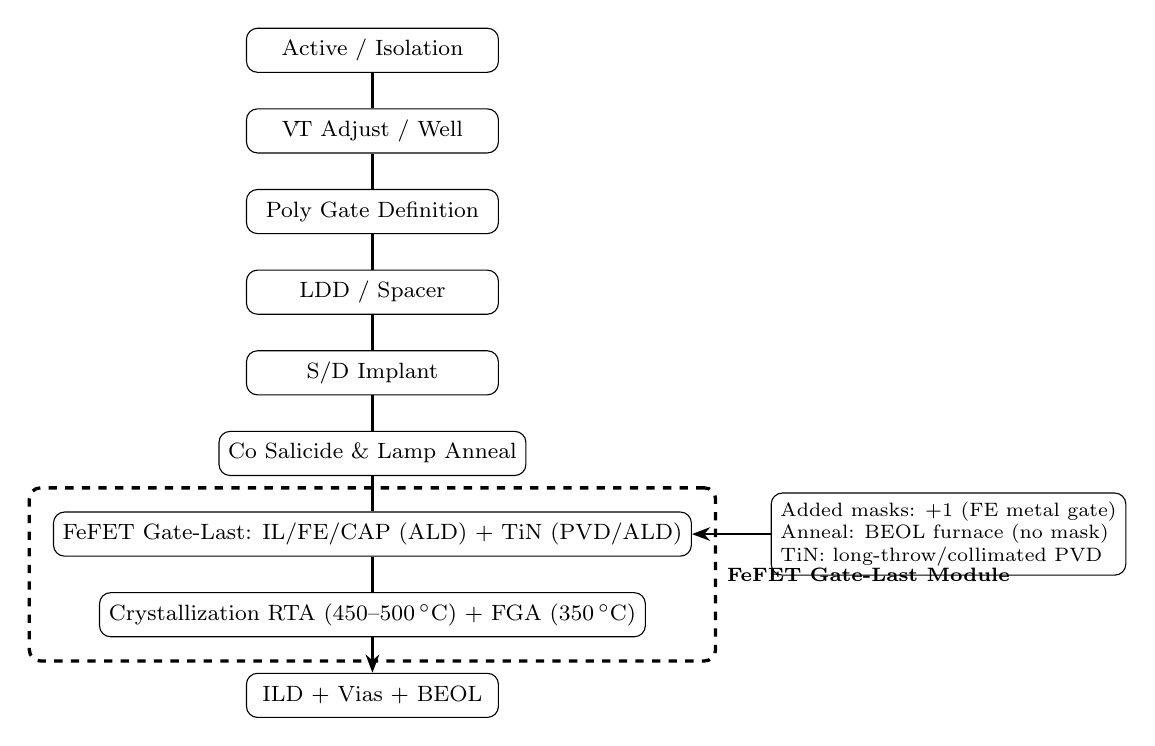
\begin{tikzpicture}[
  node distance=4.5mm,
  stage/.style={draw,rounded corners,minimum width=32mm,minimum height=5.6mm,align=center,font=\footnotesize},
  arr/.style={-{Stealth},thick},
  ann/.style={font=\scriptsize}
]
\node[stage] (act)  {Active / Isolation};
\node[stage,below=of act] (vt)  {V\!T Adjust / Well};
\node[stage,below=of vt]  (poly) {Poly Gate Definition};
\node[stage,below=of poly] (ldd)  {LDD / Spacer};
\node[stage,below=of ldd]  (imp)  {S/D Implant};
\node[stage,below=of imp]  (sal)  {Co Salicide \& Lamp Anneal};
\node[stage,below=of sal]  (fegate)  {FeFET Gate-Last: IL/FE/CAP (ALD) + TiN (PVD/ALD)};
\node[stage,below=of fegate]  (rta)  {Crystallization RTA (450--500\,\si{\celsius}) + FGA (350\,\si{\celsius})};
\node[stage,below=of rta]  (ild)  {ILD + Vias + BEOL};

\draw[arr] (act) -- (vt) -- (poly) -- (ldd) -- (imp) -- (sal) -- (fegate) -- (rta) -- (ild);

% dashed bracket to highlight FeFET module
\node[draw,dashed,very thick,rounded corners,fit=(fegate) (rta),inner sep=3mm,
      label={[ann]right:\textbf{FeFET Gate-Last Module}}] {};

% note box
\node[draw,rounded corners,align=left,font=\scriptsize,anchor=east,
      right=10mm of fegate] (note) {Added masks: +1 (FE metal gate)\\
Anneal: BEOL furnace (no mask)\\
TiN: long-throw/collimated PVD};
\draw[arr] (note.west) -- (fegate.east);
\end{tikzpicture}
\caption{Placement of FeFET module within the 0.18\,$\mu$m CMOS baseline (vertical layout).}
\label{fig:flow}
\end{figure}

% ---- Mask/step table (self-contained) ----
\begin{table}[t]
  \centering
  \caption{Added masks / process steps relative to baseline logic.}
  \label{tab:masks}
  \begin{tabular}{@{}lcc@{}}
    \toprule
    \textbf{Step} & \textbf{Mask} & \textbf{Comment}\\
    \midrule
    FE metal gate & +1 & Shared / reuse analog option route\\
    FE anneal     &  0 & Done in BEOL furnace (no extra mask)\\
    \bottomrule
  \end{tabular}
\end{table}

\subsection*{Device Stack}
TiN / Hf$_{0.5}$Zr$_{0.5}$O$_2$ (8--12\,nm, ALD) / Al$_2$O$_3$ IL (1--2\,nm) / p-Si.

\subsection*{Implementation Notes}
The 1.8\,V / 3.3\,V CMOS baseline was extended with an additional 1.8\,V FeFET option. FeFET devices are used as auxiliary elements for 1.8\,V SRAM macros, not as large-scale memory blocks. Although challenges remain regarding endurance, retention, TDDB, and yield, difficulty is reduced since large array scaling is not targeted. Integration is feasible within a legacy 0.18\,$\mu$m line by adding ALD; TiN can use existing barrier sputter (long-throw/collimated). The FeFET module is inserted after FEOL Co salicide and lamp anneal, requiring only one extra mask.

% =========================================================
% Experimental Conditions
% =========================================================
\section{Experimental Conditions}
\maybeinput{build/experimental_conditions_en.tex}

% =========================================================
% Reliability (all figures inside)
% =========================================================
\section{Reliability}
\maybeinput{build/reliability_en.tex}

% =========================================================
% Conclusion
% =========================================================
\section{Conclusion}
\maybeinput{build/conclusion_en.tex}

% ================= References =================
\bibliographystyle{IEEEtran}
\bibliography{refs}

% ================= Biography =================
\section*{Author Biography}
Shinichi Samizo received the M.S. degree in Electrical and Electronic Engineering from Shinshu University, Japan.  
He joined Seiko Epson Corporation in 1997, where he engaged in semiconductor device process development including 0.25--0.18\,$\mu$m CMOS, HV-CMOS, \textbf{DRAM}, FeRAM, and FinFET/GAA research.  
He also contributed to inkjet MEMS process development and thin-film piezo actuator design, leading to the productization of PrecisionCore printheads.  
His expertise covers semiconductor devices (logic, memory \textbf{[DRAM/FeRAM/SRAM]}, high-voltage mixed integration), inkjet actuators, and AI-based control education.

\end{document}
